\chapter{A Physical Perspective on The Rescue of Mutant CFTR}
\label{chap:perspective}

\begin{chapquote}{Deborah Marcus \cite{marcus_ouroboros}}
and take the time to remember\\
the looping bend, surged\\
began as the walking end
\end{chapquote}

\section{Introduction}

The preceding chapters have fit into some broad themes. Chapters \ref{chap:introduction} and \ref{chap:methods} outlined a philosophy of biological physics. Meanwhile, chapters \ref{chap:cftr}-\ref{chap:opening} collected molecular details about the misfunction of CFTR, to built up an understanding of the root cause of Cystic Fibrosis, and demonstrate that small molecule drugs can rescue diverse modes of CFTR misfunction. In this chapter we will tie these themes together. We will introduce a physical perspective on the rescue of mutant CFTR by potentiator drugs. A similar model could be built for corrector drugs, or even used to think about the modulation of any protein by small molecules.

We hope that this model will inform our current understanding of the action of CFTR modulators and also direct future efforts in treating the root cause of Cystic Fibrosis. We will outline specific studies motivated by this model in the next chapter.

We will begin with a brief overview of our results so far, analysing 4 rare CF-causing mutations which appear to respond to CFTR modulators even though they each have a unique molecular defect. We will then look at the molecular details of one of the best studied and most common disease causing mutations, G551D

%, and where it fits in relation to the array of other disease causing mutations. 

We will show through simple unbiased MD, that this mutation causes a disruption to the binding of ATP, resulting in a gating defect. As with previous chapters, this gating defect appears unique, sharing little in common with the other gating defects we analysed previously. This array of different disease phenotypes leads us to propose a model based on the gating energy landscape, which accounts for the rescue of unique phenotypes by a common mechanism of action. 

We will demonstrate how to use our proposed model to theratype a rare mutation, Q1291H, from the molecular level. We will show how the Q1291H mutation appears to exhibit a similar molecular phenotype to G551D, leading us to expect that it will be amenable to rescue by the same modulators. This is despite the fact that patients carrying this mutation are currently excluded from receiving modulator therapy in all jurisdictions. 

In the next chapter we will use this proposed model to assess priorities for future studies of CFTR. It is hoped that these future studies will collect the necessary quantitative information about CFTR, to fill in the missing information in our proposed model and, leading to better patient outcomes. 

%Our simulations of G551D and Q1291H appear to show a similar molecular phenotyope, even though they occur on different parts of the protein. Q1291H is an extremely rare mutation, it has not been clinicarlly characteriesd and is not approved for treatment with modulators. So, by studying a common mutation, G551D and comparing it to Q1291H we give an example of theratyping of CF mutations from the molecular level.


\section{Summary Of Rare Mutations Studied so Far}

	\begin{center}
		\includegraphics[width=\textwidth]{figures/perspective/summary.pdf}
	\end{center}
\begingroup
\captionsetup{singlelinecheck = false, justification=raggedright}
\captionof {figure}[Summary of our Rare Mutation Studies] {\textbf{Summary of our Rare Mutation Studies}}{All of the mutations analysed in this thesis so far have been largely unique. They largely occur on different domains of the CFTR protein and cause misfunction through unique set of molecular interactions. Nonetheless, all of these mutations respond, to some degree, to potentiator class modulators \cite{wong2022, wong2022a, kim2018, vanwilligen2019}. This situation demands that we tie together these results to explain how different pathogenicity can be treated by the same mechanism of action. } 
\endgroup

In chapters \ref{chap:I37R}, \ref{chap:R352Q}, \ref{chap:S945L} and \ref{chap:opening} we analysed a disease causing mutation in detail in order to understand \textit{how} it caused CFTR to misfunction. What these chapters have shown is a large diversity of molecular phenotypes. Each of these mutations appears to cause CFTR misfunction in a different way. 

%In chapters \ref{chap:I37R}-\ref{chap:opening} we demonstrated that a diverse set of molecular defects respond to CFTR modulators. Each of these defects displayed a response to CFTR potentiators. This means that even though the molecular origin of pathogenesis was unique, each defect could be treated by a common mechanism of action. 

\begin{itemize}
	\item Chapter \ref{chap:I37R} studied the novel I37R mutation on the lasso motif. These results demonstrated that pathogenesis arises from interactions between the lasso motif and the R-domain. This caused a class III gating defect, which was responsive to both potentiators and correctors \cite{wong2022}. 
	\item Chapter \ref{chap:R352Q} studied the R352Q mutation on TMD1, to show how a conductance class defect may arise from the deletion of a positive charge in the inner vestibule of CFTR. This mutation was found to cause a class IV conduction defect, which responded to potentiators \cite{wong2022a}.
\item Chapter \ref{chap:S945L} studied the S945L mutation on TMD2. Our simulations showed how a stable network of hydrogen bonds allows the channel to fold and gate correctly. When this set of hydrogen bonds was broken, it led to class II and III folding and gating defects. This mutation was found to benefit from combination therapies, thus deriving some benefit from correctors as well as potentiators.  
\item Chapter \ref{chap:opening} studied the R334W mutation on TMD1. By using a dilated conformation of CFTR, we found that the deletion of a positive charge in selectivity filter of CFTR lead to a class IV conductance defect. Previous studies in the literature demonstrated that this mutation also benefits from combination therapies, indicating that the protein is amenable to modulation by both correctors and potentiators. 
\end{itemize}

The molecular phenotypes in each mutation were unique. They occur in different parts of the CFTR protein and each had a different set molecular interactions which resulted in pathogenesis. What is thus remarkable is that the \textit{in vitro} evidence accompanying these computational these studies all demonstrate that these mutations are responding to the same modulators, albeit with differing efficacies. Each mutation we simulated responded to the mechanism of action of potentiators to some degree. These results, in combination with the knowledge that 174 other mutations have been shown to respond \textit{in vitro} to a combination therapy, lead us to expect that the majority of missense mutations will be amenable to treatment via CFTR modulators \cite{trikafta_FDA_info}. It is merely a problem of choosing the correct ones for each patient.

Here we will propose a rational basis for action of modulators and eventually, quantitatively predict whether a mutation ill respond to a given modulator. At the time of writing, there does not exist sufficient computational power to complete this model---but in the next chapter we will outline the necessary steps for future studies. The completion of this model will lead to a rational basis for the choice of modulators, specific to each. 

In this chapter we will demonstrate the application of this rational basis. By briefly studying a common class III gating mutation, G551D, and how it fits into the overall classification of CF-causing mutations. Using this model we will show how to compare the molecular modes of misfunction between G551D and Q1291H, leading us to predict that they will respond to the same modulators. 

\section{Simulating the Common G551D Gating Mutation}

	\begin{center}
		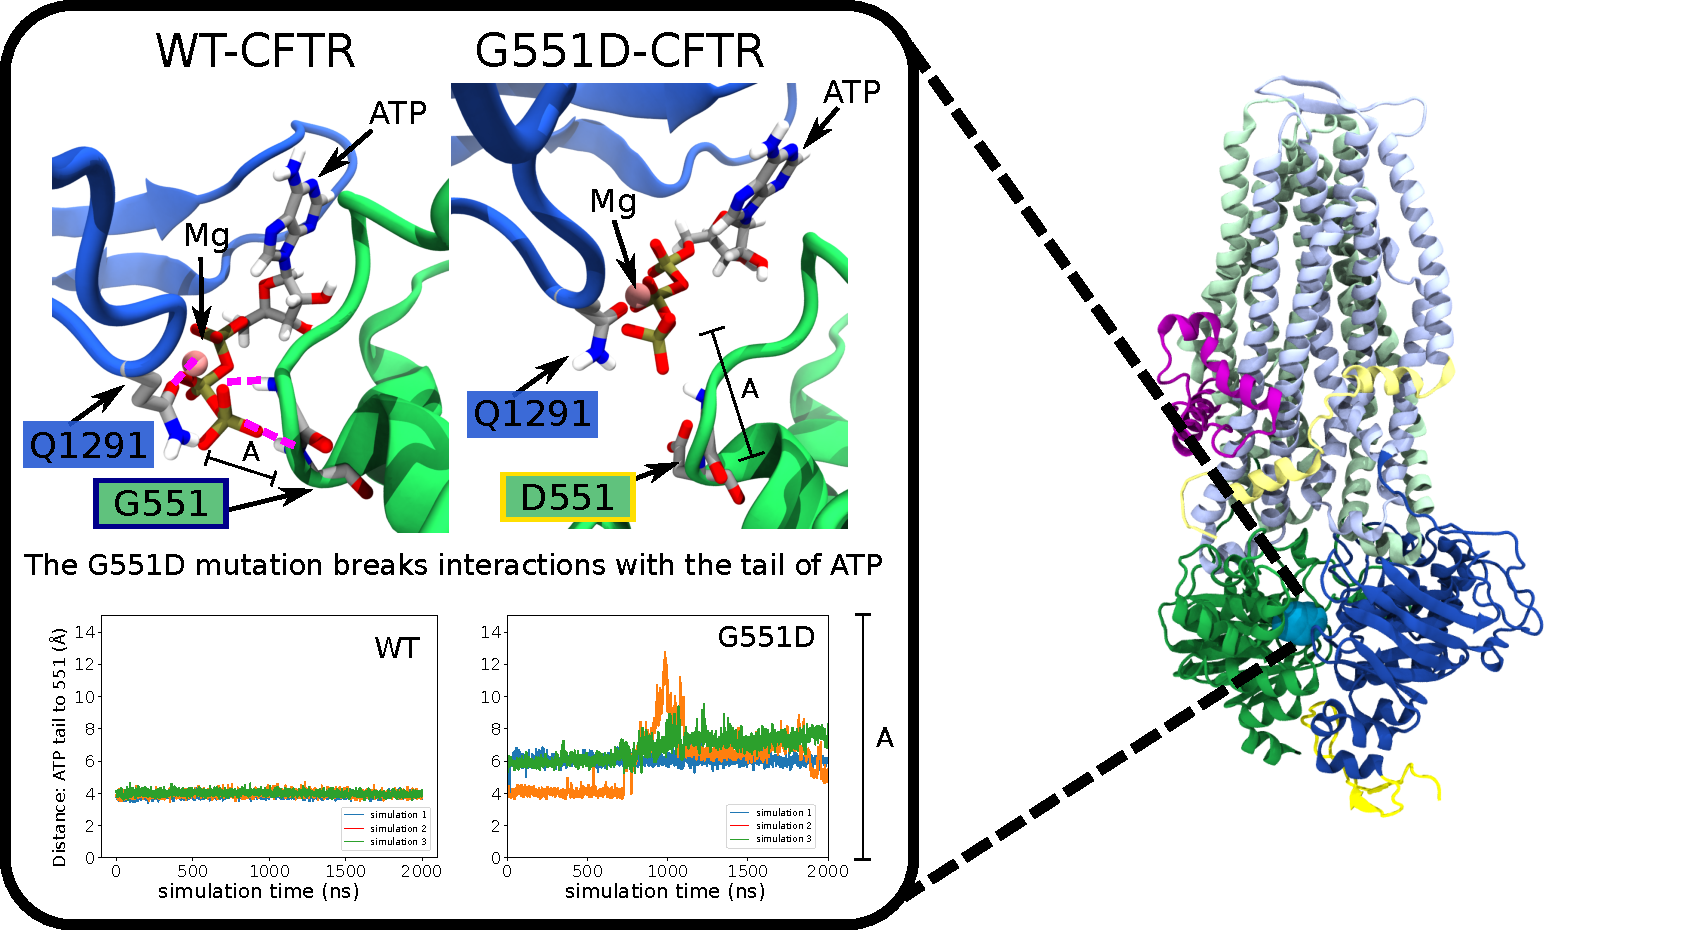
\includegraphics[width=\textwidth]{figures/perspective/G551D.pdf}
	\end{center}

\begingroup
\captionsetup{singlelinecheck = false, justification=raggedright}
\captionof {figure}[Pathogenesis in G551D-CFTR] {\textbf{Pathogenesis in G551D-CFTR}}{G551D-CFTR exhibits the prototypical gating phenotype \textit{in vitro} \cite{bompadre2007, wang2020}. A) The mutation is located on NBD1, in the vicinity of site 1, the hydrolytic ATP+Mg binding site. B) MD simulations indicate that this mutation disrupts ATP-binding, as the amide groups on the backbone of G550 and G551 stabilize the phosphate tail of the bound ATP molecule. These links were found to be disrupted in the mutant.} 
\label{G551D_results}
\endgroup

Here, we will briefly continue the theme of previous chapters, with a simple MD study to understand pathogenesis in a common class III gating mutation, G551D \cite{li1996}. This will place the mutation in context with the rest of our work. This gating mutation occurs in NBD1, a domain we have not yet studied in the work of this thesis (Figure \ref{G551D_results}A). It has an important role historically, as it was the candidate for high-throughput screening in order to discover potentiator class drugs \cite{vangoor2009}. This means that G551D is a good candidate for comparison with other rare mutations, if we wish to find other mutations which might also respond to potentiators.

Our simulations discovered that the G551D mutation disrupts critical hydrogen bonds which stabilise the phosphate tail of ATP in site 1. Given the importance of ATP binding to the gating cycle of CFTR, these observations are a clear rational basis for the confirmation of G551D as a gating defect \cite{}. 

The above molecular defect in G551D-CFTR is a again unique in relation to the other mutations we have studied. Nonetheless, this is another example of a set of characteristic molecular defects may be treated by CFTR modulators. In the next section we will take a broader view, to understand what kind of molecular defects have been rescued by modulators so far.

\section{The Many Molecular Modes of Misfunction in CFTR}

Throughout the literature and this thesis, we have found many molecular modes of misfunction, every mutation we have looked at seems relatively unique. Hence, it is unlikely that the course classification of 6 classes conventionally used to understand CFTR mutants can be used to theratype patients. A more granular, molecular understanding will be needed to choose which mutations can be rescued by specific modulators. 

In Figure \ref{granular_classification} we have surveyed the available literature to sketch out a more complete, more granular classification of different mutations. Observe in this figure how we have identified 16 different structural and functional modes of CFTR misfunction, as opposed to the conventional 6. These classes themselves are quite broad. For example the category, ``NBD folding" contains contain dozens of mutations not listed---F575Y, S492F, R560S, R1066C, S1128F, to name a few \cite{awatade2019, lopes-pacheco2016, casals1997, cotten1996, penmatsa2009}. As before, each of these mutations likely have their own characteristic molecular fingerprints which give result in pathogenesis. It will take some work to split up this category further, to make it more meaningful when choosing modulators which target specific mutations.

The complexity in Figure \ref{granular_classification} shows some of the nuance within CF pathogenesis. In order to make this summary more manageable and more meaningful, we will propose a physical model with which to understand the modulation of gating class CFTR mutants. 

\begin{landscape}
\begin{figure}
	\begin{center}
	%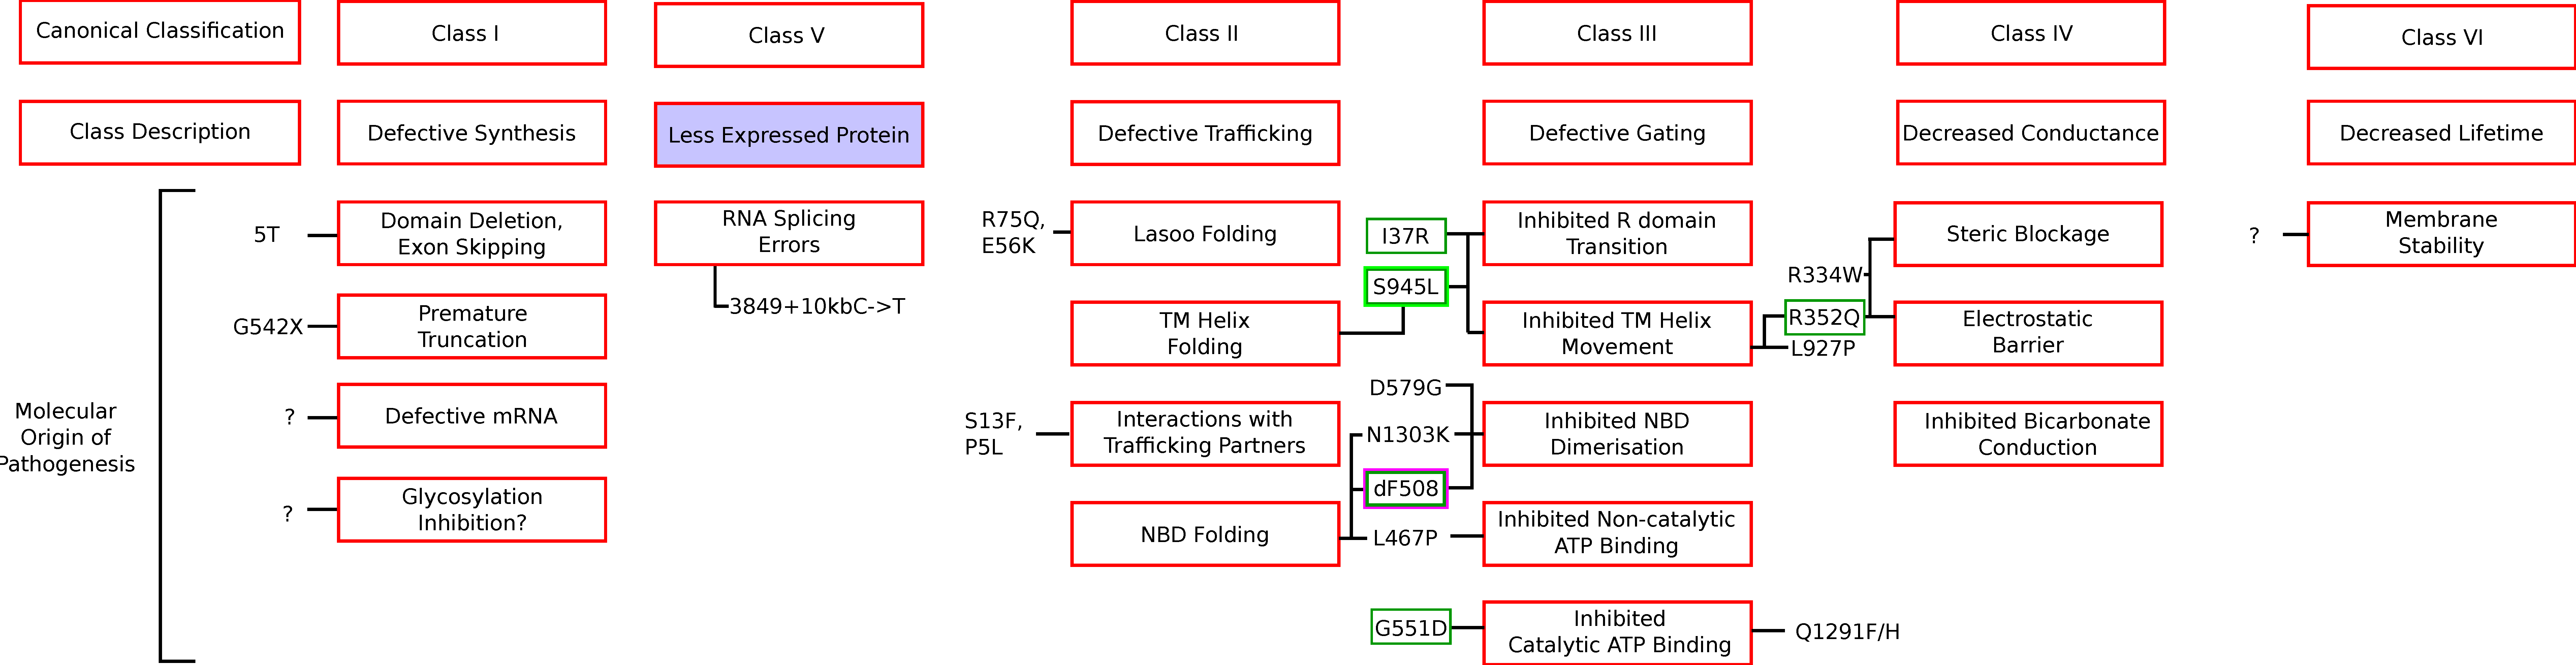
\includegraphics[angle=270,origin=c,width=0.38\textwidth]{figures/classes_mutations.pdf}\\
	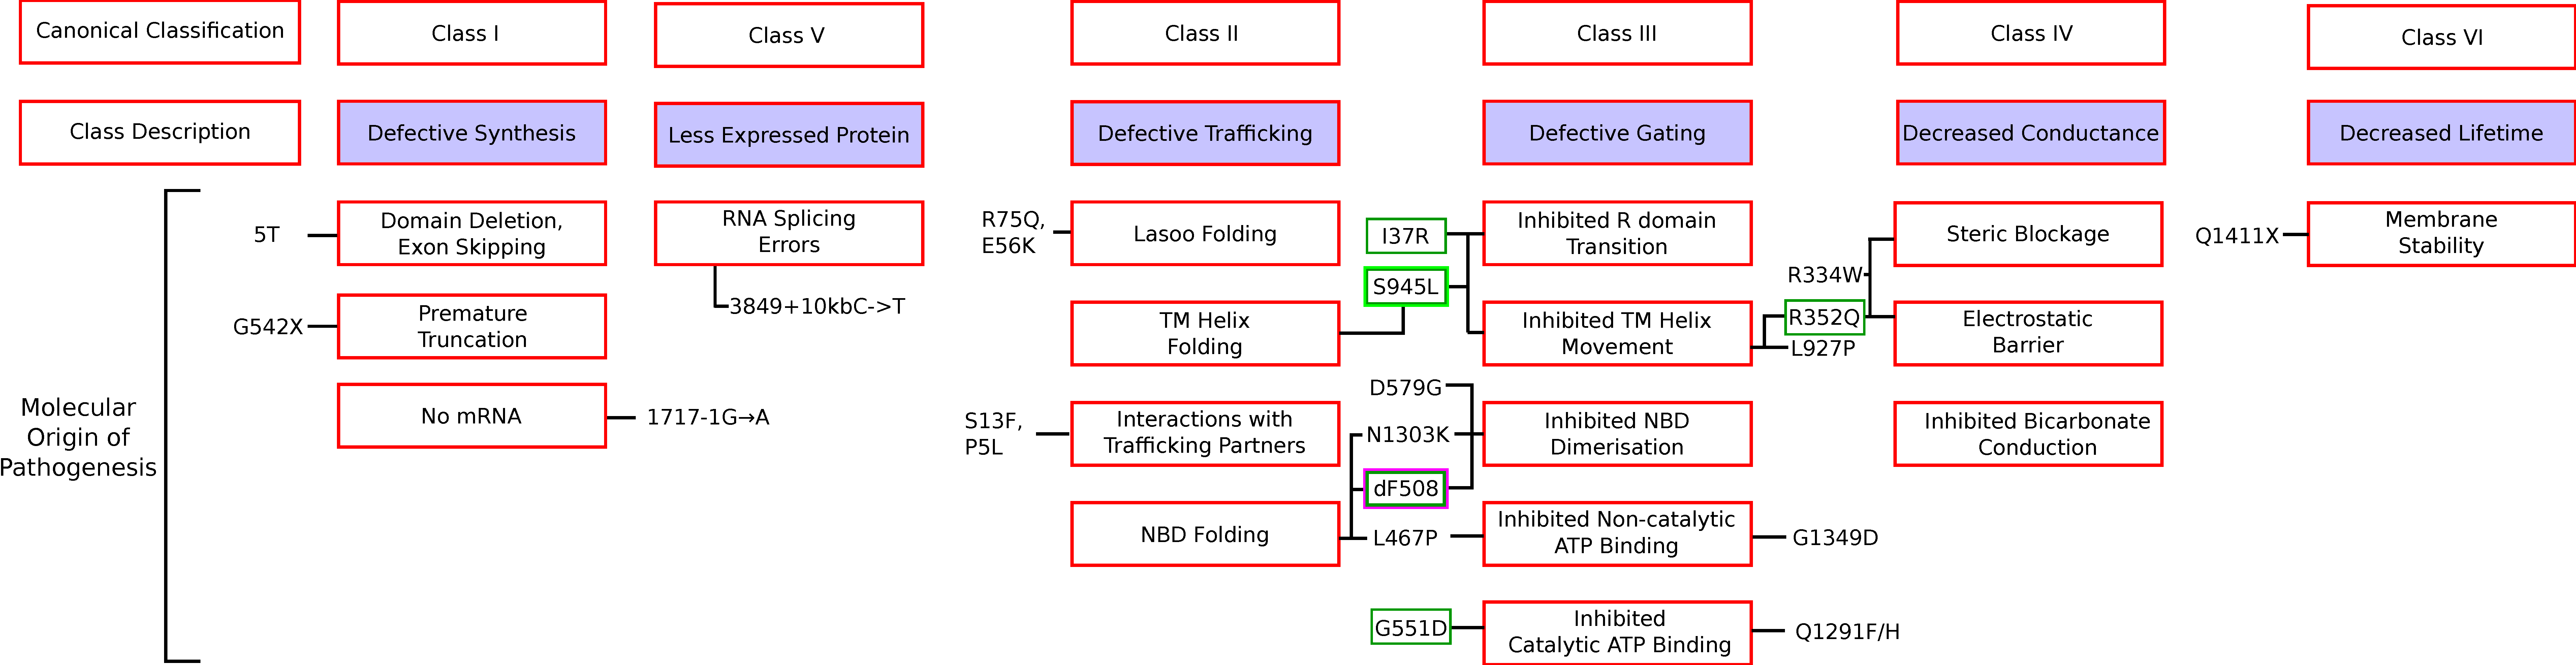
\includegraphics[width=1.5\textwidth]{figures/perspective/classes_mutations.pdf}\\
	\end{center}
	\captionsetup{singlelinecheck = false, justification=raggedright}
	\caption[Granular grouping of CF pathogenesis]{\textbf{Granular Grouping of Cystic Fibrosis Causing Mutations}{ Conventionally, molecular CF phenotypes are grouped into 6 classes. These classes, while useful in a clinic, are quite broad. They struggle to reflect that molecular misfunction of misfunction can arise from many interactions within CFTR. By realising that classification into a given class can be due to different factors we can gain a more complete picture of the molecular cause of CF by delineating the molecular fingerprint of each mutation. The links drawn in this figure were inferred from a combination of sources in the literature, our own findings and from a mutation's location in the CFTR protein \cite{bompadre2007, gong2004, wong2022, vangoor2009, vangoor2014, hoffmann2018, thelin2007, gene2008, trikafta_website, phuan2018, ensinck2022}. The inhibited bicarbonate conductance class was included to highlight that this there are few molecular studies which have sought to understand the molecular effects of different mutations on the conduction of bicarbonate. }
	}

	\label{granular_classification}
\end{figure}
\end{landscape}

\section{A Physics Motivated Approach to Personalised Medicine in Cystic Fibrosis}
Observe in Figure \ref{granular_classification} how mutations which cause misfunction different ways may respond to the same modulators. For example, as we have shown in detail I37R and G551D occur on different domains of CFTR, resulting in different kinds of pathogenesis. Despite this, they can both be rescued by potentiator class drugs. In order to explain these results in this chapter I will propose a conceptual framework which explains how these drugs are able to treat such diverse molecular phenotypes. This model would appear to suggest that patients with rare missense mutations are likely respond to the right choice of CFTR modulator. These implications may also inform the design of future CFTR modulators and this will be discussed in the next chapter. 

\begin{figure}
	\begin{center}
		\begingroup
	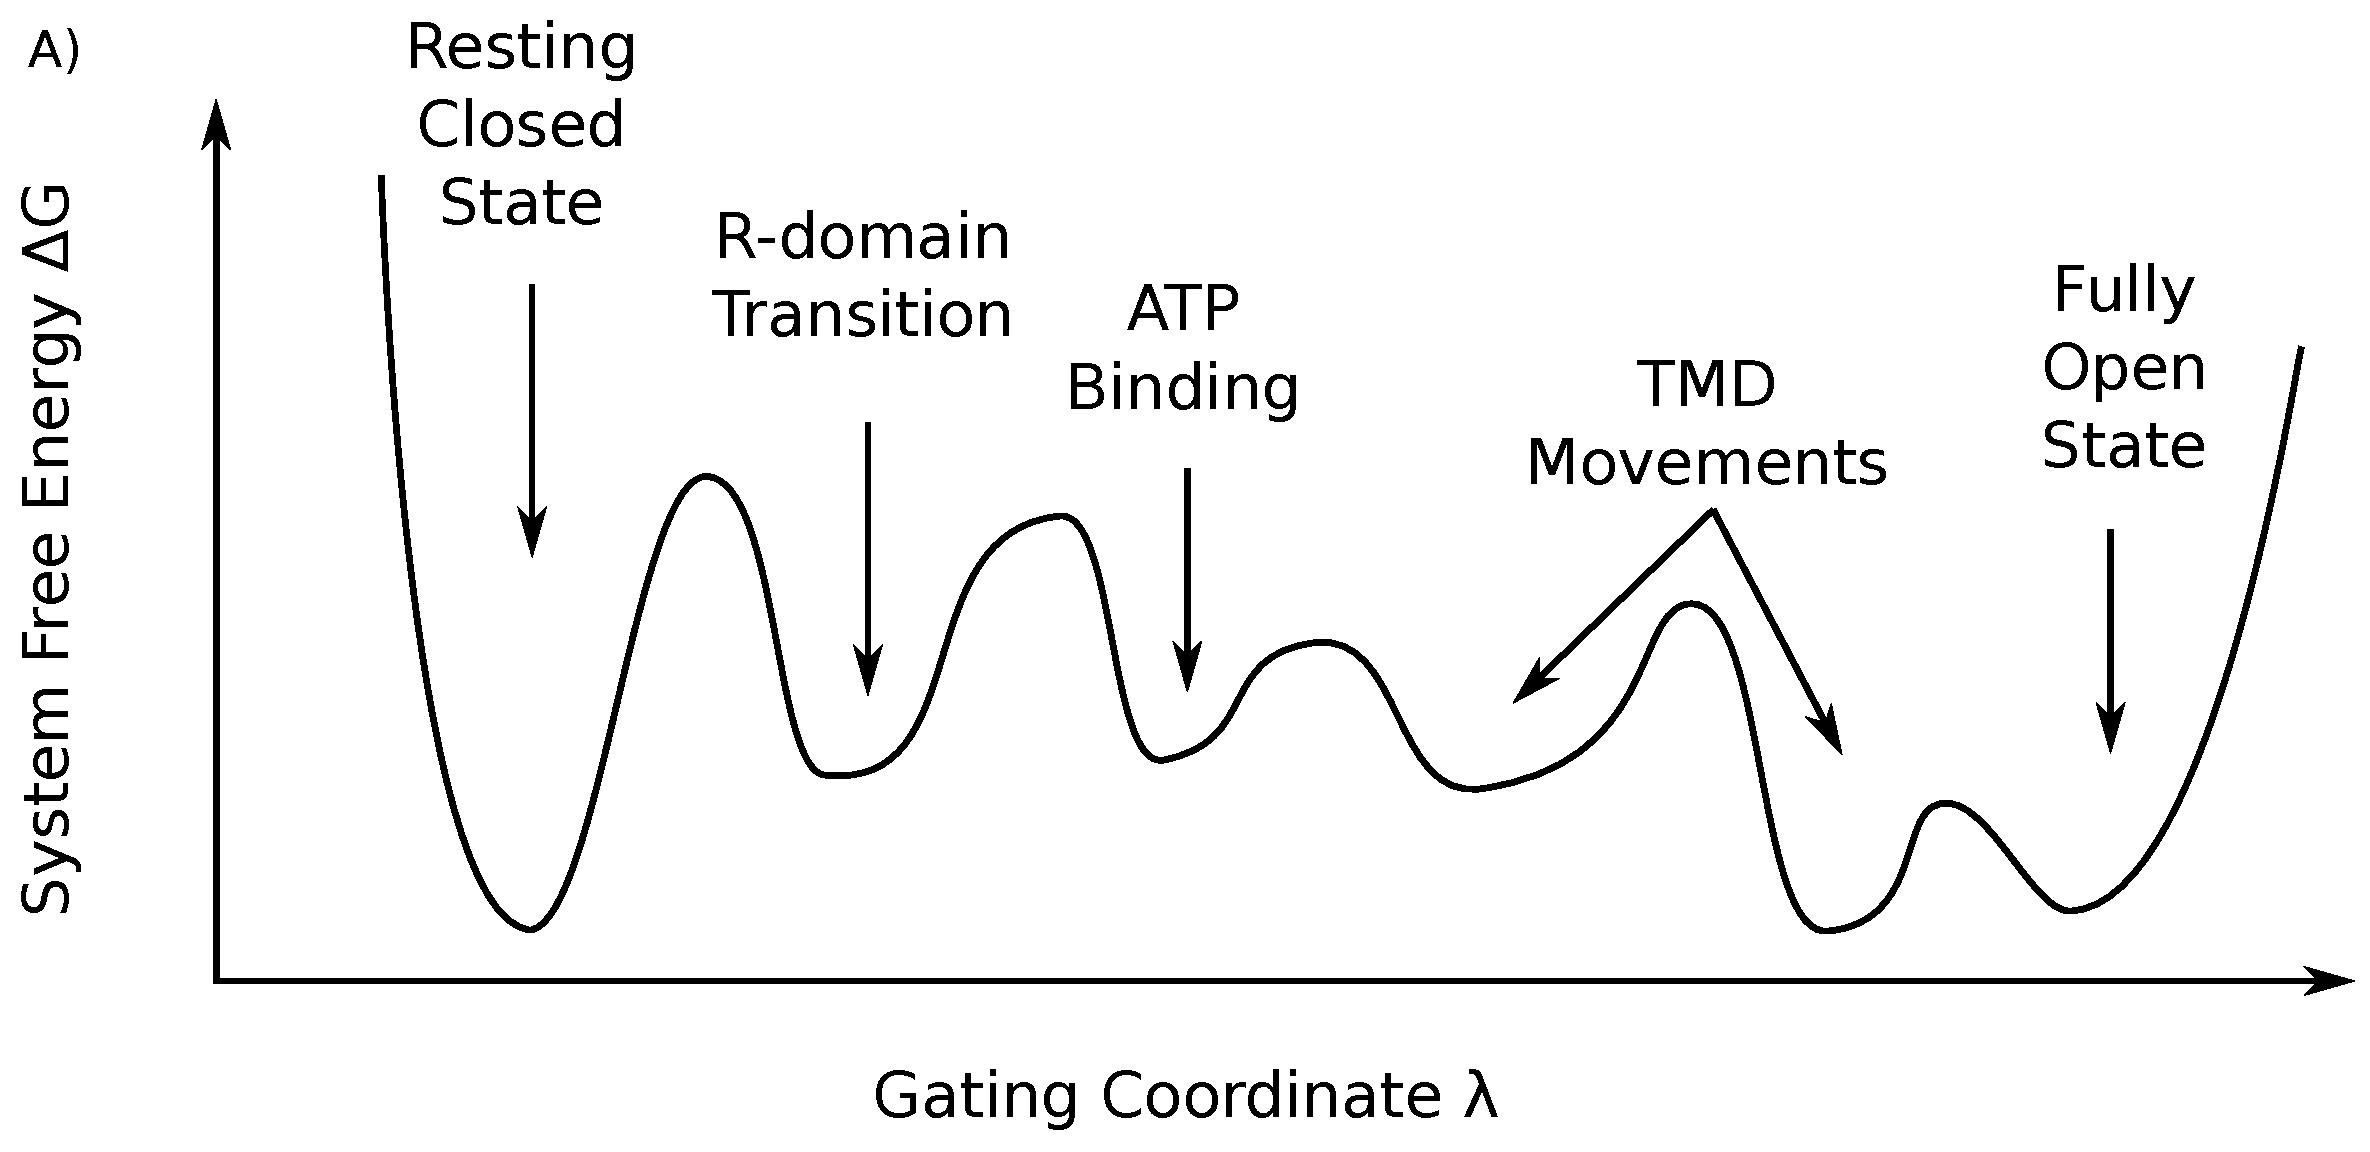
\includegraphics[width=0.6\textwidth]{figures/perspective/drug_landscape_1.pdf}\\
	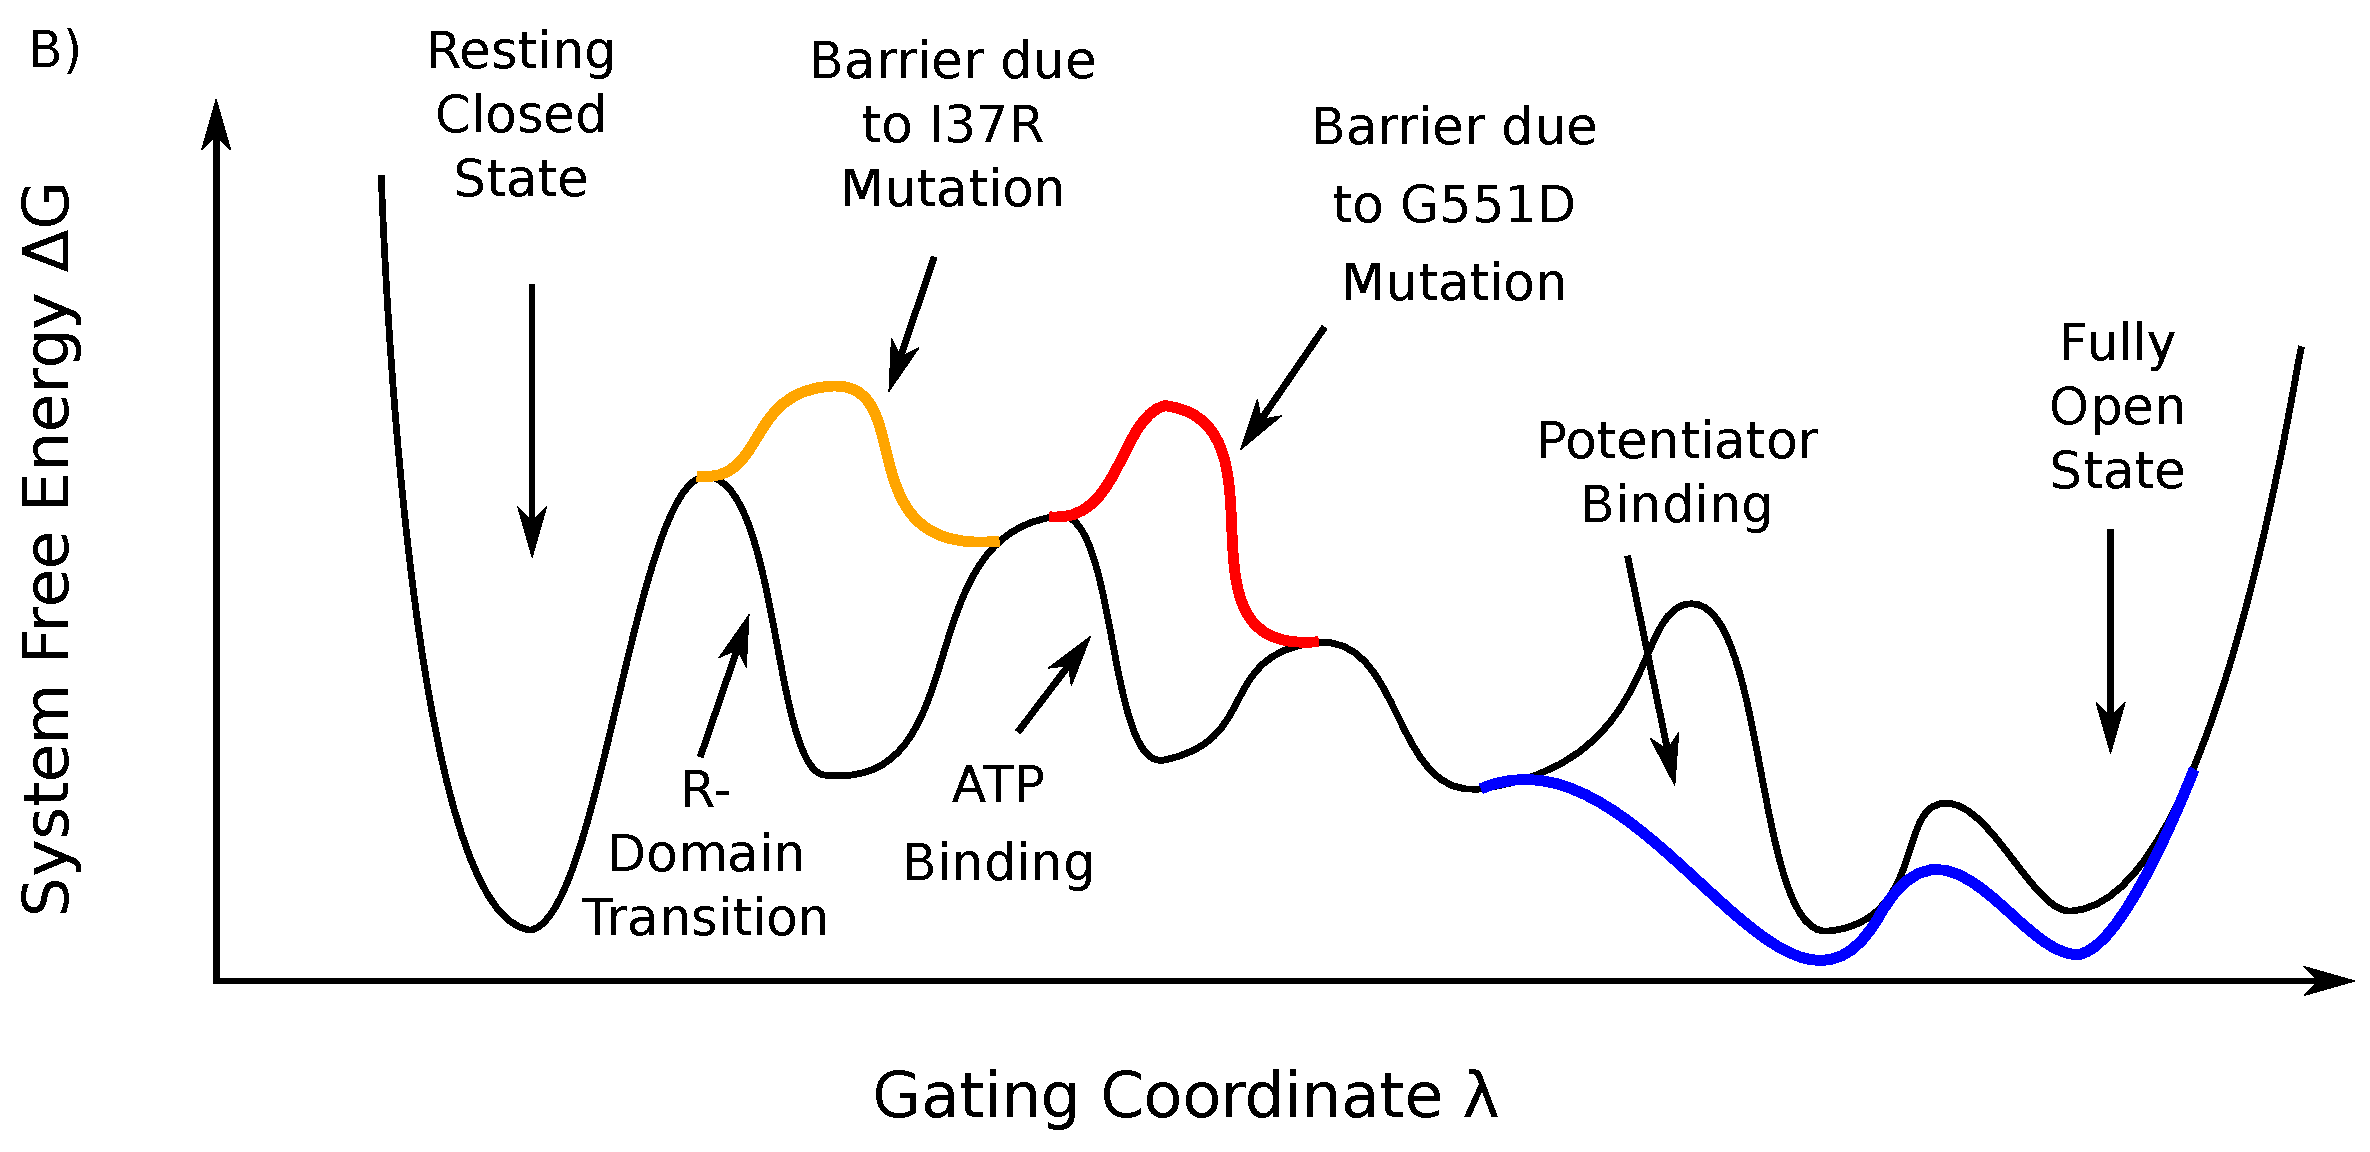
\includegraphics[width=0.6\textwidth]{figures/perspective/drug_landscape_3.pdf}\\
		\endgroup
	\end{center}
	\begingroup
	\captionsetup{singlelinecheck = false, justification=raggedright}
	\captionof{figure}[Conceptual Framework for the Pathogenesis of Mutations and The Action of Potentiators]{\textbf{Conceptual Framework for the Pathogenesis of Mutations and The Action of Potentiators}{ A) The transition between the resting closed state and fully open state of CFTR can be visualised as a movement through an energy landscape. Along this transition various events must occur, such as the movement of the R-domain, ATP-binding and the rearrangements of the different domains of CFTR. Each of these events will have an energetic cost and payoff, giving rise to peaks and troughs in the energy landscape of the transition. The relative heights of peaks and troughs here are for illustrative purposes only, but quantitative techniques to calculate them will have important implications for the treatment of CF and drug discovery. B) Gating class CF-causing mutations give rise to pathogenic barriers in this energy landscape which prevent the transition to an open state. They may arise in different parts of the energy landscape. For example, we have shown that G551D causes a disruption to the binding of ATP, while in chapter \ref{chap:I37R}, we saw a gating defect arise in I37R-CFTR from the misregulation of the position of the R-domain. This demonstrates how pathogenesis can arise in many different ways in CFTR. Furthermore, accompanying \textit{in vitro} studies of these mutations demonstrated that these unique mutations each respond to potentiator class modulators. This indicates that CFTR potentiators are bringing down \textit{other} barriers in this energy landscape in order to compensate for these mutations. By understanding \textit{where} mutations are causing gating inhibition and \textit{how} drugs are accounting for the deleterious energetics, we can begin to build a molecular basis for the choice of modulators, tailored to each mutation.}}
	\label{drug_action_model}

	\endgroup
\end{figure}

The model in Figure \ref {drug_action_model} has been proposed to explain the action of potentiators in the treatment of gating defects. It was forma tooled this way because gating transition is simpler, there are many well studied events which we can visualise in our model energy landscape, like ATP binding and pore formation by the TMDs. Hence, we have built our model with a focus on this aspect of protein function. Nonetheless, the conceptual basis of this model is transferable to CFTR folding as well. As we elucidate the folding pathway of CFTR, we will also be able to build up a similar model for the action of correctors \cite{krainer2018, kleizen2021, kleizen2020, fiedorczuk2022}. 

Currently a range of missense mutations are recommended for treatment by Trikafta but many more are excluded from receiving this treatment due to a lack of testing. The above model suggests that when a patient carrying such a rare mutation does not respond to modulator therapy, it is unlikely that the lack of a response is due to the inability of these modulators to rescue the function of CFTR. From the perspective of protein physics, $\Delta$F508 is likely to cause a greater effect to CFTR much more than most missense mutations \cite{bahia2021}. In this way it makes little sense not to screen most patients carrying missense mutations for a response to modulators. Should a patient's cells not respond to modulators I believe it is more likely that this is due to the broader heterogeneous response to modulators found in many CF patients \cite{boyle2014, donaldson2018, keating2018, matthes2018}, rather than the failure of modulators to act on mutant CFTR. Hence, the pre-clinical, patient specific approach like the one employed by the collaborators of this thesis is most appropriate for the treatment of CF. 

To aid this work, we have contributed to the molecular understanding of CF with our model. We will now demonstrate how to could be used in future to theratype a rare mutation. We have specifically chosen a poorly studied mutation from our dataset to demonstrate the power of the model we now have in hand. 

\section{Theratyping Q1291H-CFTR With Atomic Precision}

Through our molecular modelling we noticed another defect, Q1291H appears to produce a similar molecular defect to G551D, even though it is located on a different domain of CFTR (NBD2 as opposed to NBD1). G551D is much more common than Q1291H, and so patients carrying the former may access potentiators. However, Q1291H is extremely rare, with only 30 CFTR alleles of this mutation recorded in the CFTR2 database, this mutation is poorly understood clinically \cite{cftr2}. Samples with this mutation are in the biobank of Sydney Children's hospital, taken from a CF afflicted patient. 

Because of their heterozygous alleles, and the rarity of the Q1291H mutation, this patient is currently excluded from receiving modulator therapy. As with our previous studies, we propose that computational results can compliment, and in this case, predict the results of patient specific \textit{in vitro} assays. Hence, we have undertaken computational modelling in order to understand the molecular defect caused by the Q1291H mutation. 

These results show that both G551D and Q1291H disrupt ATP binding at site 1. Further, since we know that this kind of disfunction is amenable to rescue by CFTR modulators in the case of G551D, we would expect that patients carrying the Q1291H mutation would also benefit from modulator therapy. These results lead us to expect that the Q1291H mutation would benefit from modulator therapy, due to its similarity to the G551D mutation. Although computational modelling is not sufficiently advanced to make a recommendation for any patient without \textit{in vitro} studies, this situation is not uncommon for those carrying rare forms of CF, and so we recommend that this mutation be tested in patient specific assays, as it has a high likelihood to translate to clinical practice. 

This recommendation is further strengthened by the fact that the Q1291R mutation at the same site, which is likely more deleterious than Q1291H, is reccomended for treatment with both potentiators and combination therapies \cite{trikafta_website, trikafta_FDA_info, kalydeco_FDA_approval}.

The preceding chapters have given technical and molecular details about the cause of Cystic Fibrosis by rare genetic mutations, and further demonstrated that these mutations may be treated by existing small molecule drugs. The unique molecular fingerprint of each mutation indicates that in order to deliver better outcomes to patients a more personalised approach is necessary in the choice of medication. 


%There is no reason to beleive that even in patients who do not show benefit from modulator therapy that the drugs are for some reason not reaching the CFTR protein. In fact, they seem to metabolise the drugs at teh same rate as patients who do. The success of preclinical models indicates that the problem is the cellular level and not at the level of organs or tissues. There is probably some genetic or cellular component that has not yet been identified which, once addressed, could bring the benefits of modulators to these patients.




\begin{figure}
	\begin{center}
		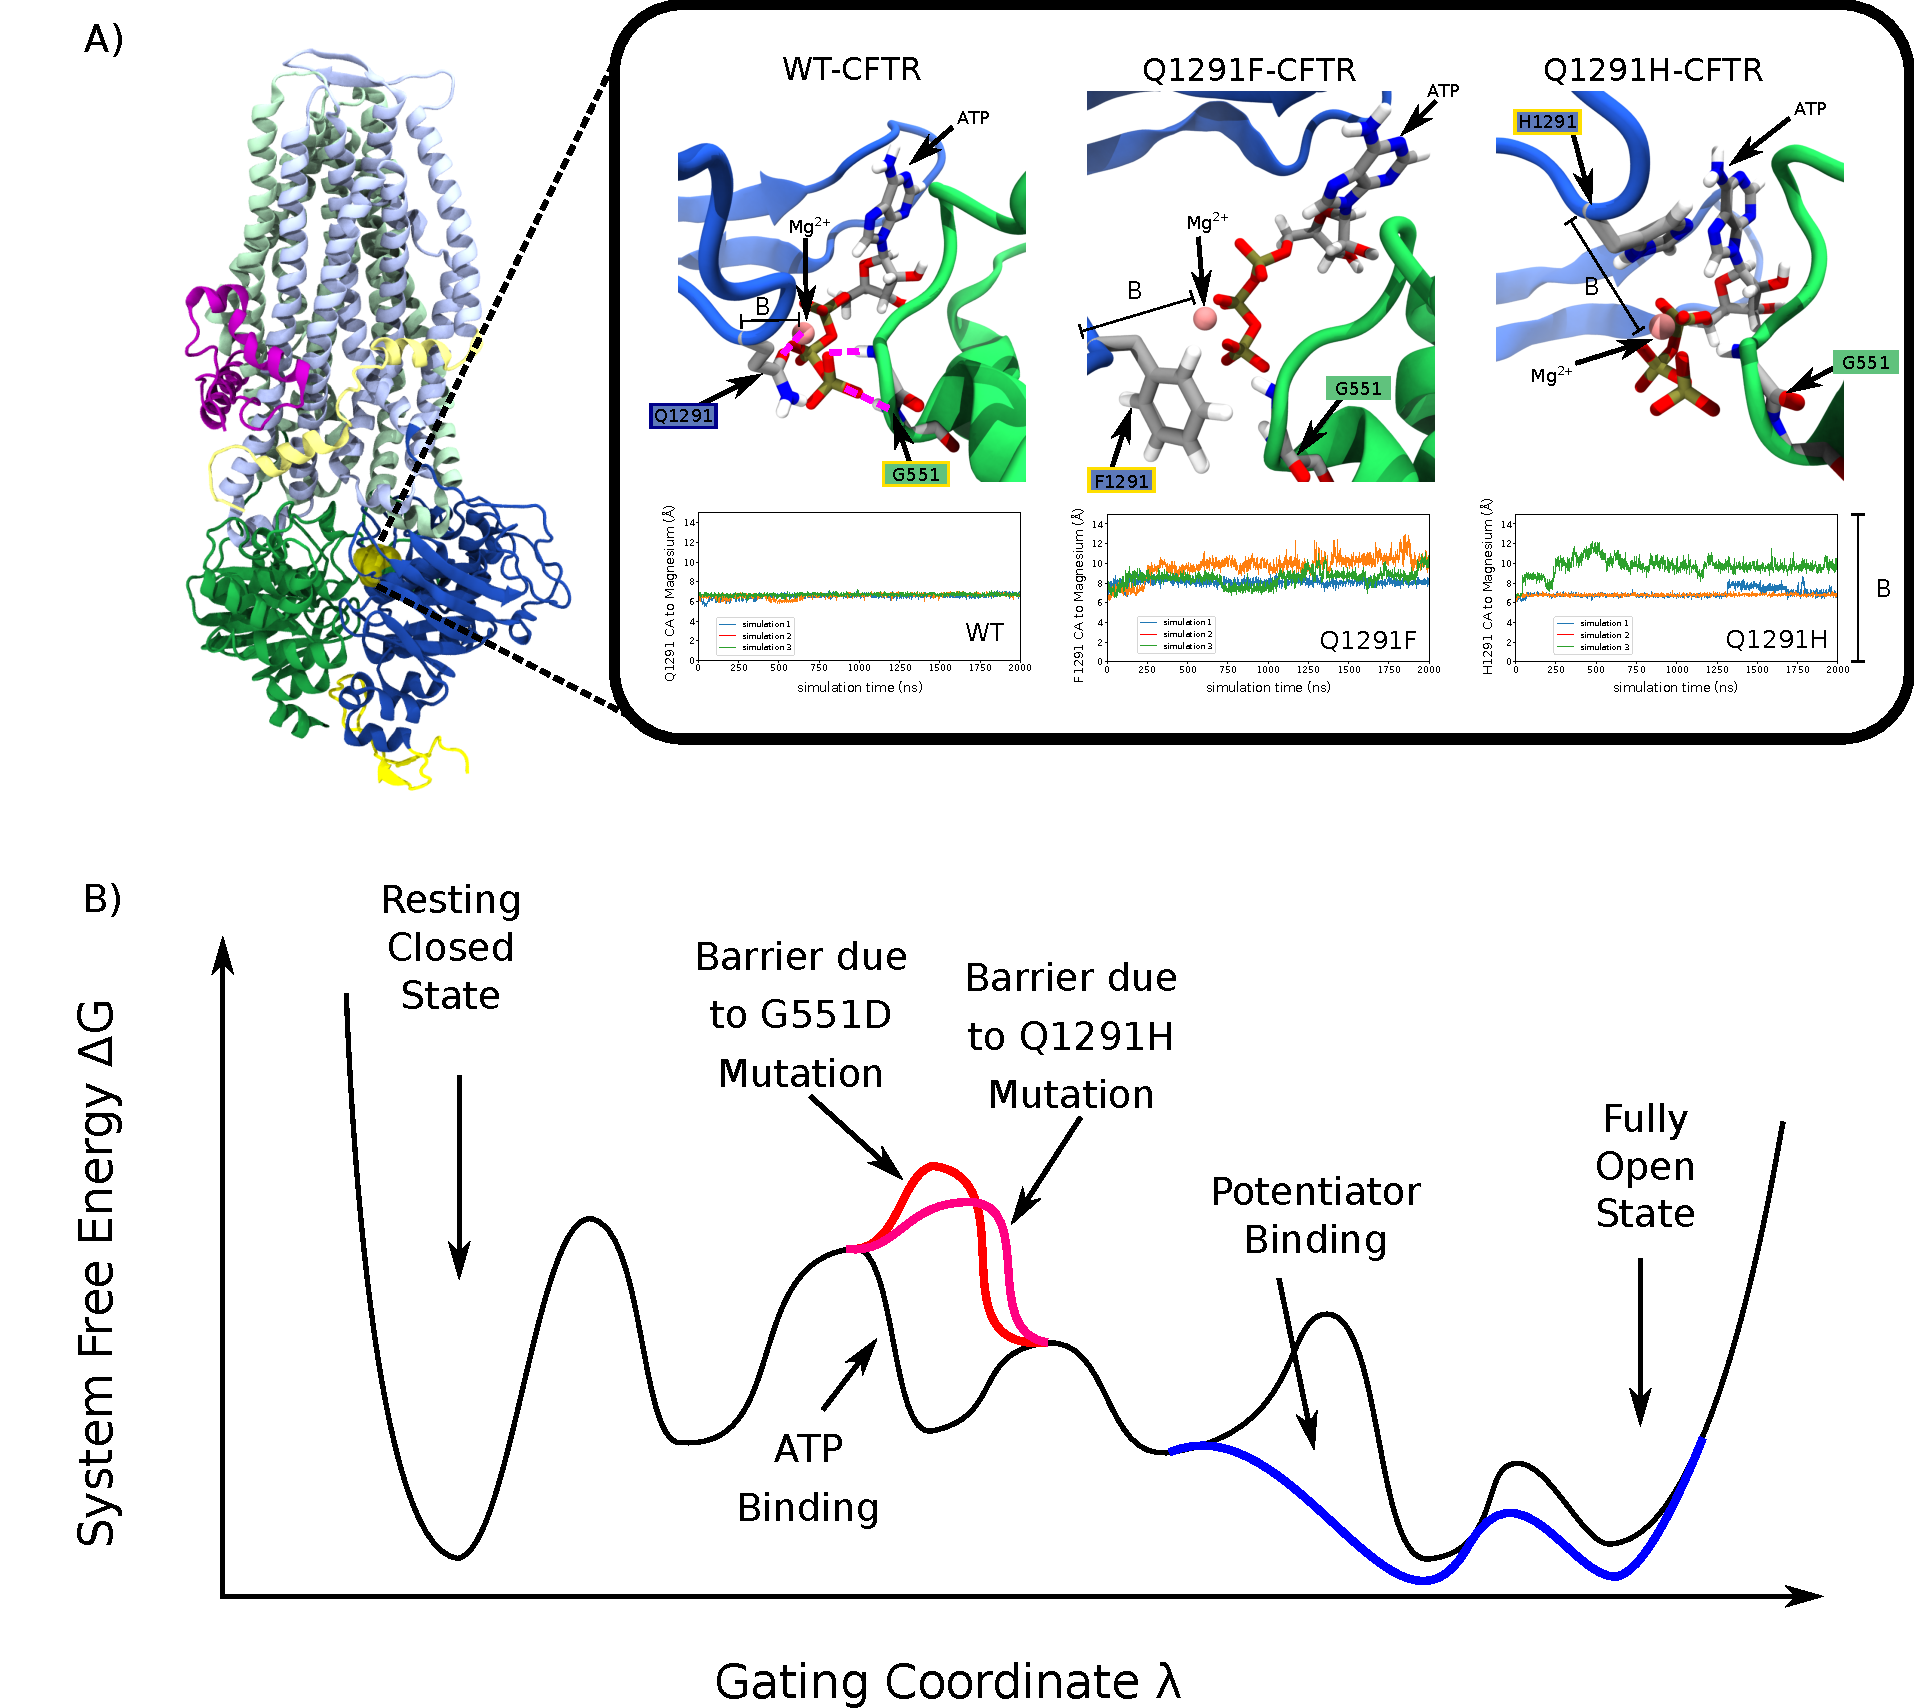
\includegraphics[width=\textwidth]{figures/perspective/Q1291.pdf}
	\end{center}
	\captionsetup{singlelinecheck = false, justification=raggedright}
	\caption[Pathogenesis in Q1291H-CFTR]{\textbf{Pathogenesis in Q1291H-CFTR}{A) The Q1291H mutation occurs on NBD2, in the vicinity the catalytic ATP binding site. B) It appears as though this mutation also causes disruption to the binding of this ATP molecule, much like G551D. Data from simulations Q1291F is also included, as it more reliably produces the molecular perturbation which we expect is characteristic of the Q1291H mutation. \textit{In vitro}, the two mutations produce similar behaviour and this is confirmed in our simulations. }}

\end{figure}


%These drugs are clinically efficacious \cite{VanGoor2014} on several mutants with some curious exceptions like N1303K. I suggest the following mechanism for their action. I suspect a similar analogy exists for the action of the correctors. WT-CFTR exhibits a natural landscape with kinetic barriers in the transition between the closed and open states. A gating class mutation to CFTR will introduce a kinetic barrier in the pathway of this conformational transition. What these drugs do is reduce a barrier in the existing conformational landscape of CFTR. This compensates for the barriers introduced by the mutation. j


\section{Summary}
In summary, the important findings from the 4 prior modelling studies, and the presented study of G551D have lead us to propose a model for the rescue of gating class mutations by small molecule drugs. This model sought to account for the fact that we have seen 5 unique defects all respond to potentiator drugs, and we expect a similar model could be drawn for folding class defects. This that many disease causing alleles will respond to modulator therapy, even though they are currently excluded from these treatments by regulatory agencies. 

In recent years there have been a slew of rare CF-causing genotypes discovered in populations with low rates of Cystic Fibrosis compared to Caucasians. These genotypes from Asia and the Middle East are often ultra-rare leading, to poor outcomes for these patients \cite{}. 

In the next chapter, we will give some examples of a set of \textit{in silico} and \textit{in vitro} studies which can be used to complete this model.

\section{Method Details}
Simulation methodologies employed in this chapter were identical to those employed in chapter \ref{chap:S945L}. All MD simulations in this chapter were carried out at a physiological temperature of 310K (37$^o$C).
